\section{Prelude}

\subsection{Prerequisite Notation}


Though the course has no specific mathematical prerequisites, a general familiarity with the set of integers and some of its basic properties will be assumed. We collect here some useful facts and notations that will appear from time to time throughout the course. We'll add more as the need arises.
\begin{enumerate}
\item 
Notations for important sets of numbers
\begin{itemize}
\item 
$\mathbb{Z} = \{\ldots -2,-1,0,1,2,\ldots\}$ (the integers)
\item 
$\mathbb{N} = \{0,1,2,\ldots\}$ (the non-negative integers, a.k.a. the natural numbers)
\item 
$\pint=\{1,2,3,\ldots\}$ (the positive integers)
\end{itemize}
\item 
Important facts about numbers
\begin{itemize}
\item 
The Least Number Principle: If $X$ is a nonempty subset of \nnint, then $X$ has a least element.
\item 
Principle of Mathematical Induction: If $X$ is a subset of \nnint, and $0\in X$, and for every $i$, if $i\in X$, then $i+1\in X$, then $X=\nnint$.
\item The Pigeonhole Principle: If you distribute $m$ pigeons into $n$ pigeonholes and $m>n$, then some hole contains more than one pigeon.
\end{itemize}
\item Unique Factorization into Primes: Recall that $p\in\pint$ is \emph{prime} if and only if $p\neq1$ and $p$ is divisible only by $1$ and $p$. Every $n\in\pint$ with $n\neq 1$ can be written uniquely as $p_1^{a_1}\cdots p_n^{a_n}$ where each $p_i$ is prime and each $a_i\geq 1$. 
\end{enumerate}

\subsection{A Combinatorial Warmup}

Combinatorics is, roughly, the part of mathematics which deals with counting things. Its techniques are general, and its results tangible. Throughout this book, we will use combinatorial problems as concrete examples of problems which can be considered and solved by means of logical techniques. To get our feet wet, let's consider the following principle and question. 

\begin{principle}\label{PHP}
\textbf{The Pigeonhole Principle}: If you distribute $m$ pigeons into $n$ pigeonholes and $m\geq n+1$, then some hole contains at least two pigeons.
\end{principle}

\begin{example}
\label{numDiv}
Is there a numerically diverse group of Philadelphians?
\end{example}

(We call a group of people numerically diverse if no two people in the group have the same number of friends in the group - we assume groups are of size at least two and that friendship is always mutual.) 

We will demonstrate that the answer is no by an application of the Pigeonhole Principle. 
\begin{proof}
Suppose we have a group $G=\{1,\ldots,n\}$ of $n$ people (we use numerals to name the people for privacy concerns). For brevity, let's write $p_{ij}$ to signify that $i$ is a friend of $j$. We assume friendship is symmetric, that is, if $p_{ij}$, then $p_{ji}$, for all $i,j\in G$, and irreflexive, that is, it is not the case that $p_{ii}$, for all $i\in G$. Let's write $f(i)$ for the number of friends of $i$, that is, the number of $j$ such that $p_{ji}$. Since friendship is irreflexive, the possible values of $f$ are the $n$ numbers $0, 1,\ldots,n-1$. We are thinking of these values as the pigeonholes for application of the principle \ref{PHP} and the members of $G$ as being placed in these holes by $f$. We want to argue that the value of $f$ must agree on at least two members of $G$. But so far, since we have $n$ members of $G$ and $n$ pigeonholes into which they are sorted by $f$, we may not yet draw that conclusion via principle \ref{PHP}. But now we consider the question, ``can $f$ really take all the values from $0$ to $n-1$?'' In particular, can it take on both the value $0$ and the value $n-1$? We argue that the answer is no. Suppose that there is some $i$ with $f(i)=0$, that is, for every $j$, it is not the case that $p_{ji}$. Then, by symmetry, for every $j$, it is not the case that $p_{ij}$. So, if $i$ has no friends, then the maximum number of friends of any $j$ is $n-2$, that is, $f$ cannot take on the value $n-1$. Thus, the possible values of $f$ are the $n-1$ numbers $0,\ldots,n-2$. But now, by principle \ref{PHP}, we can conclude that $f$ takes on the same value for at least two members of $G$. This concludes our argument that there cannot be a numerically diverse group of Philadelphians. 
\end{proof}

\begin{aside}
The above argument presupposes that there are finitely many Philedelphians. In fact, the theorem does not hold if we allow Philadelphia to have infinitely many people. As an exercise, try to describe a numerically diverse group of infinitely many Philadelphians. 
\end{aside}

The Pigeonhole Principle can take on a more general form, the \emph{Mean Pigeonhole Principle}, which is as follows:

\begin{principle}\label{MPHP}
\textbf{The Mean Pigeonhole Principle}: If you distribute $m$ pigeons into $n$ pigeonholes and $m\geq k\cdot n +1$, then some hole contains at least $k+1$ pigeons. 
\end{principle}

\begin{aside}
Note that Principle \ref{PHP} is just the special case of Principle \ref{MPHP} for $k=1$.
\end{aside}

\begin{example}
Say a group of people has three-mutuality if it contains either a group of three mutual friends or a group of three mutual strangers. How large a group of people can lack three-mutuality?
\end{example}
We show that the largest such group has five members. To do this, we will give an example of a pattern of friendship among a group of five people that lacks three-mutuality, and show that every pattern of friendship among six or more people has three-mutuality. To show that every friendship pattern on six or more people lacks three-mutuality, we will use the Mean Pigeonhole Principle. 

\begin{proof}
The diagram below shows a ``friendship pentagon''. Nodes represent people, and an edge between people represents friendship. It is easily checked that the diagram lacks 3-mutuality. 

\begin{center}
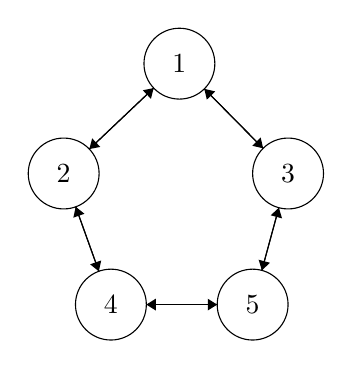
\begin{tikzpicture}[scale=0.15]
\tikzstyle{every node}+=[inner sep=0pt]
\draw [black] (41.5,-11) circle (3);
\draw (41.5,-11) node {$1$};
\draw [black] (31.7,-20.3) circle (3);
\draw (31.7,-20.3) node {$2$};
\draw [black] (50.7,-20.3) circle (3);
\draw (50.7,-20.3) node {$3$};
\draw [black] (35.7,-31.4) circle (3);
\draw (35.7,-31.4) node {$4$};
\draw [black] (47.7,-31.4) circle (3);
\draw (47.7,-31.4) node {$5$};
\draw [black] (39.32,-13.07) -- (33.88,-18.23);
\fill [black] (33.88,-18.23) -- (34.8,-18.05) -- (34.11,-17.32);
\draw [black] (33.88,-18.23) -- (39.32,-13.07);
\fill [black] (39.32,-13.07) -- (38.4,-13.25) -- (39.09,-13.98);
\draw [black] (32.72,-23.12) -- (34.68,-28.58);
\fill [black] (34.68,-28.58) -- (34.88,-27.66) -- (33.94,-27.99);
\draw [black] (34.68,-28.58) -- (32.72,-23.12);
\fill [black] (32.72,-23.12) -- (32.52,-24.04) -- (33.46,-23.71);
\draw [black] (49.92,-23.2) -- (48.48,-28.5);
\fill [black] (48.48,-28.5) -- (49.17,-27.86) -- (48.21,-27.6);
\draw [black] (44.7,-31.4) -- (38.7,-31.4);
\fill [black] (38.7,-31.4) -- (39.5,-31.9) -- (39.5,-30.9);
\draw [black] (38.7,-31.4) -- (44.7,-31.4);
\fill [black] (44.7,-31.4) -- (43.9,-30.9) -- (43.9,-31.9);
\draw [black] (48.59,-18.17) -- (43.61,-13.13);
\fill [black] (43.61,-13.13) -- (43.82,-14.05) -- (44.53,-13.35);
\draw [black] (43.61,-13.13) -- (48.59,-18.17);
\fill [black] (48.59,-18.17) -- (48.38,-17.25) -- (47.67,-17.95);
\draw [black] (48.48,-28.5) -- (49.92,-23.2);
\fill [black] (49.92,-23.2) -- (49.23,-23.84) -- (50.19,-24.1);
\end{tikzpicture}
\end{center}


Next, we show that every group of $n \geq 6$ people must have 3-mutuality. Again, write $p_{ij}$ to denote that $i$ is a friend of $j$.  

Let $G=\{1,\ldots,6\}$ and sort the five people $2,\ldots,6$ into two pigeonholes according to the truth value, true ($\top$) or false ($\bot$) of $p_{12},\ldots,p_{16}$. That is, sort people $2,\ldots,6$ into two groups, one group which are all friends of $1$, and one group all of which are not friends with $1$. By Principle \ref{MPHP}, one of these holes, suppose it's the $\top$ one, contains at least three members of $G$.

Now, either two of these are friends, in which case they, together with $1$ form a collection of three mutual friends, or none of them of friends, in which case they themselves form a collection of three mutual strangers. The argument is analogous, in the case that three members of $G$ were sorted into the $\bot$ pigeonhole. 
\end{proof}

\begin{aside}
We might wonder whether every natural number $n$ has a $k$ such that every group of at least size $k$ has $n$-mutuality. This happens to be true (try proving it!). The \emph{Ramsey number} $R_{m, n}$ is the least $k$ such that every set of $k$ people must have either a group of $m$ mutual friends or $n$ mutual strangers. In the previous example, we shoed that $R_{3, 3} = 6$. Higher ramsay numbers are much harder to compute. We know that $R_{4, 4} = 18$. $R_{5, 5}$ is currently known to be between $43$ and $48$. $R_{6, 6}$ is somewhere between $102$ and $165$. 

As an exercise, prove that $R_{m, n} = R_{n, m}$ for all $m, n$.

``Suppose aliens invade the earth and threaten to obliterate it in a year's time unless human beings can find the Ramsey number for red five and blue five. We could marshal the world's best minds and fastest computers, and within a year we could probably calculate the value. If the aliens demanded the Ramsey number for red six and blue six, however, we would have no choice but to launch a preemptive attack.'' - Paul Erdos
\end{aside}

Love differs from friendship in that there are narcissists (so we can't assume the relation is irreflexive) and is not always requited (so we can't assume the relationship is symmetric). This difference between friendship and love allows the existence of numerically diverse groups of lovers, that is, groups where each person in the group loves a different number of people in the group. Consider, for example, a group of four people, $\{1, 2, 3, 4\}$. Suppose that $1$ doesn't love anyone, $2$ loves $1$, $3$ loves both $1$ and $2$, and $4$ loves all of $1,2$, and $3$, and that this exhausts all the love among our group of four. We achieve numerical diversity at the sacrifice of requital. 

\begin{center}
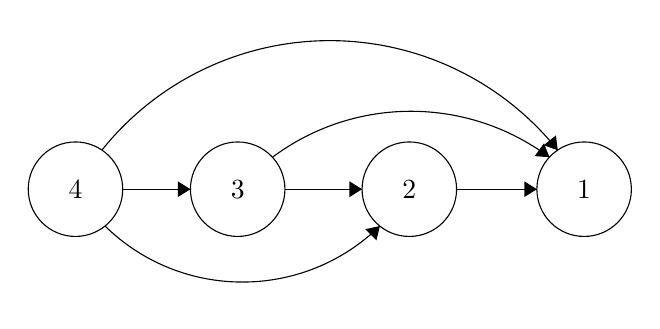
\begin{tikzpicture}[scale=0.2]
\tikzstyle{every node}+=[inner sep=0pt]
\draw [black] (53.2,-20.3) circle (3);
\draw (53.2,-20.3) node {$1$};
\draw [black] (42.1,-20.3) circle (3);
\draw (42.1,-20.3) node {$2$};
\draw [black] (31.2,-20.3) circle (3);
\draw (31.2,-20.3) node {$3$};
\draw [black] (20.9,-20.3) circle (3);
\draw (20.9,-20.3) node {$4$};
\draw [black] (45.1,-20.3) -- (50.2,-20.3);
\fill [black] (50.2,-20.3) -- (49.4,-19.8) -- (49.4,-20.8);
\draw [black] (34.2,-20.3) -- (39.1,-20.3);
\fill [black] (39.1,-20.3) -- (38.3,-19.8) -- (38.3,-20.8);
\draw [black] (33.405,-18.273) arc (126.74959:53.25041:14.7);
\fill [black] (51,-18.27) -- (50.65,-17.39) -- (50.06,-18.2);
\draw [black] (40.229,-22.635) arc (-45.59639:-134.40361:12.474);
\fill [black] (40.23,-22.64) -- (39.31,-22.84) -- (40.01,-23.55);
\draw [black] (22.578,-17.817) arc (141.31542:38.68458:18.54);
\fill [black] (51.52,-17.82) -- (51.41,-16.88) -- (50.63,-17.51);
\draw [black] (23.9,-20.3) -- (28.2,-20.3);
\fill [black] (28.2,-20.3) -- (27.4,-19.8) -- (27.4,-20.8);
\end{tikzpicture}
\end{center}

How many different patterns of love might obtain among a group of four people $\{1,2,3,4\}$? Let's recycle the sentence letters and use $p_{ij}$ to signify the statement that $i$ loves $j$; note that 16 sentence letters would be required to record all the relevant statements. Since each pattern of love among $1,2,3,4$ is determined by assigning one of the truth values $\top$ or $\bot$ to each of these 16 sentence letters, we can conclude that the number of such patterns is $2^{16}$. Why? Because there are two assignments to $p_{11}$ and for each of these, there are two assignments to $p_{12}$, and thus $2\cdot 2 = 2^2$ assignments to them jointly (this observation is given the exalted title, ``The Product Rule''). Thus, by iterating application of the product rule another fourteen times, we arrive at the conclusion that there are $2^{16}$ possible truth assignments to the 16 sentence letters. 

\begin{aside}
    $2^{16} = 65536$. It's kind of amazing that there are as many as 65,536 different potential love-scenarios at a table for four!
\end{aside}

Friendship, as compared to love, is relatively tame in terms of the number of scenarios that might arise. Let's return to using $p_{ij}$ to indicate that $i$ and $j$ are friends. In virtue of the fact that friendship is symmetric and irreflexive, a friendship-scenario is determined by assigning one of the truth values $\top$ or $\bot$ to each of the 6 sentence letters $p_{ij}$, for $1\leq i < j\leq 4$. Hence, there are only $2^6=64$ possible patterns of friendship among the group of four, less than 1/1000 of the number of potential love-scenarios. 

\begin{aside}
In general, how many possible friendship scenarios are there among a group of $n$ people? Well, every pair can either be friends or not friends, so there are $2^{num\_pairs}$ possibilities. How many pairs are their, in terms of $n$? 
\end{aside}

\newpage

\subsection{Review}
\begin{mdframed}[linewidth=1]
\section*{Concept Review}
\begin{itemize}
    \item \textbf{Pigeonhole Principle}: If you have $n + 1$ pigeons and you try to fit them all into $n$ holes, then there has to be at least one hole with $k > 1$ pigeons. 

    \item \textbf{The Mean Pigeonhole Principle}: If you distribute $m$ pigeons into $n$ pigeonholes and $m\geq k\cdot n +1$, then some hole contains at least $k+1$ pigeons. 

    \item \textbf{Product Rule}: If there are $n$ ways to do a first action and $m$ ways to do a second action, there are $n\cdot m$ ways to do both action 1 and action 2. 
\end{itemize}
\end{mdframed}


\newpage
\begin{mdframed}[linewidth=1]
\section*{Problems}
\begin{enumerate}
    \item Let $X$ be a set, $|X| = n$ (we write $|X|$ for the size of the set $X$). How many subsets does $X$ have? 

    \item How many subsets of even size does a set $X$ of size $n$ have?

    \item Prove that the Cartesian plane cannot be colored using only two colors (Red/Blue) such that all points 1 unit away from each other are different colors. 

    \item Prove that for any set of $n \geq 2$ numbers, there are $2$ numbers whose difference is divisible by $n - 1$. 

    \item Show that for any $n \in \mathbb{N}$, there is a number $k$ whose base ten numeral contains only ``$5$''s and ``$0$''s such that $k$ is divisible by $n$.  
\end{enumerate}
\end{mdframed}

\newpage
\begin{mdframed}[linewidth=1]
\section*{Solutions}
\begin{enumerate}
    \item There are $2^n$ many subsets of a set of size $n$. To see why this is the case, note that every element of the set can be either in or not in any given subset. Hence there are two choices for each of the $n$ elements of the set, and by the product rule $2^n$ choices in total. 

    \item $2^{n-1}$. Consider any nonempty subset $Y$ of $X$. Pick one element (let's call it $y$) in $Y$ and remove it from $Y$ to create a new subset $Y'$. Note that exactly one of $Y$ and $Y'$ are even: the inclusion of exlusion of $y$ corresponds to the one even and one odd subset. In this way we have associated each even subset with an odd one, and vice versa. Hence there are the same number of even and odd subsets. Since there are $2^n$ total subsets, it follows that there are $2^n/2 = 2^{n-1}$ ones of even size. 

    \item Consider an equilateral triangle with unit-length sides. We have three points pairwise one-unit apart and only two colors. The answer follows by application of the pigeonhole principle. 

    \item Note that there are $n - 1$ remainders when dividing by $n - 1$. Hence by the pigeonhole principle two of our $n$ numbers must have the same remainder when divided by $n - 1$. Their difference is divisible by $n - 1$. 

    \item Consider the first $n + 1$ elements of the set $\{5, 55, 555...\}$. We know from above that this set has two numbers whose difference is divisible by $n$. Note that the difference of any two numbers in this set is written using only $5$s and $0$s.

\end{enumerate}
\end{mdframed}